\documentclass{article} % For LaTeX2e
\usepackage{nips15submit_e,times}
\usepackage{hyperref}
\usepackage{url}
\usepackage{graphicx}
\usepackage{float}
\usepackage{amsmath,amssymb}
%\documentstyle[nips14submit_09,times,art10]{article} % For LaTeX 2.09

\DeclareMathOperator{\E}{\mathbb{E}}

\title{Bagging Deep Q-Networks}

\author{
Jamis Johnson, Lance Legal, Angus Ding \\
Department of Computer Science\\
Columbia University \\
New York, NY\\
\texttt{[jamis.johnson,lwl2110,ad3180]@columbia.edu} \\
}

% The \author macro works with any number of authors. There are two commands
% used to separate the names and addresses of multiple authors: \And and \AND.
%
% Using \And between authors leaves it to \LaTeX{} to determine where to break
% the lines. Using \AND forces a linebreak at that point. So, if \LaTeX{}
% puts 3 of 4 authors names on the first line, and the last on the second
% line, try using \AND instead of \And before the third author name.

\newcommand{\fix}{\marginpar{FIX}}
\newcommand{\new}{\marginpar{NEW}}

%\nipsfinalcopy % Uncomment for camera-ready version

\begin{document}

\maketitle

\begin{abstract}
Recent advancements by DeepMind in leveraging convolutional neural networks to 
represent the state space in Q-learning have dramatically improved the performance 
of algorithmic game playing, outperforming nearly all competing algorithms across 49
Atari 2600 games. In this paper, we propose a straight forward, distributed method for 
increasing the efficacy of deep Q-network agents thorugh the well-known ensemble algorithm,
boostrap aggregation. We have developed software to orchestrate the deployment, training, 
and testing of this method on a cluster of GPU optimized, Amazon Web Service EC-2 
virtual machines. We provide results demonstarting the effectiveness of training time
on performance as well as ensemble size to performance.
\end{abstract}

\section{Overview}
Q-networks have been shown to outperform 43 state-of-the-art agents across a 
diverse array of 49 Atari 2600 games, often by extreme margins.

\subsection{Deep Q-networks}
Q-learning is a long-standing, model-free reinforcement learning algorithm used to find 
an optimal action-selection policy[1]. Deep Q-networks are a novel approach to 
Q-learning in which deep convolutional neural networks are used to reduce high-dimensional 
raw input to a set of possible actions[2]. The convolutional neural network approximates the 
optimal action-value function

\[
Q^*(s,a) = \max_{\pi} \E \left[ r_t + \gamma r_{t+1} \gamma^2 r_{t+2} + \dots | s_t = s, a_t = a, \pi \right]
\]

which is the maximum sum of discounted rewards at time $t$. It is quite common 
to approximate $Q^*$ using a linear approximator, but in this case a 
nonlinear convolutional neural network is used such that, given $\theta$ weights, 
$Q(s,a;\theta) \approx Q^*(s,a)$. Spatial, convolutional neural networks have drastically increased 
the accuracy of image recognition tasks in recent years are therefore a natural fit as a 
state-space function approximator of raw image data[3,4,5,6,7].

\subsubsection*{Memory replay}
DeepMind emplyed a biologically-inspired memory replay mechanism that was integral
to the success of Q-networks. Experiences, $e_t = (s_t,a_t,r_t,s_{t+1})$, are stored 
at every time step $t$, where data set $ D_t = \{ e_{1}, \dots, e_{t} \} $. 
Q-learning updates are applied during learning on uniformly sampled experiences, 
with the loss function

\[
L_i(\theta_i) = \E_{(s,a,r,s') \sim U(D)} \bigg[ 
    \left( r + \gamma \max_{a'} Q(s',a';\theta^-_i) - Q(s,a;\theta)\right)^2 
\bigg]
\]

$\theta_i$ are the parameters to the Q-network and $\theta^-_i$ are the parameters used 
in the previous iteration to calculate the target.

\subsubsection*{Network architecture}
A straightforward network architecture was chosen, presumably to prop up the 
generality of deep Q-networks. The input layer receives a 84 X 84 X 4 image produced
by a preroccesing step $\phi$ which is in place to handle Atari 2600 artifacts such as 
flickering, a phenomenon that occurs because certain sprites are placed on odd or even 
numbered frames. The hidden layers are layer out as follows. First: convolves 32 filters, 
using an 8 X 8 filter, and a stride of 4; Second: 64 filters, a 4 X 4 filter, and a stride 
of 2; Third: 64 filters, a 3 X 3 filter, and a stride of 1. Each layer is followed by a 
rectified nonlinear layer, $max(0,x)$. The last hidden layer is fully connected with 512
rectified units, and the final output layer is a fully-connected linear layer with an output
per available action.


\subsection{Bagging}
Bootstrap aggregation is a standard technique for improving the stability
and performance of statistical classifiers[8].
It is commonplace to employ this method when modeling using decision trees, but has 
also been shown to produce good results when applied to artificial neural networks[9,10].

Bagging is a process of averaging across an ensemble of classifiers $f^{*n}(x)$, where $n \in [1,N]$
and training data consists of $N$ Bootstrap samples, such that

\[
f_{bag}(x) = \frac{1}{N} \sum_{n=1}^{N} f^{*n}(x)
\]

An intuitive way to think about bagging is: "the wisdom of crowds."

\subsubsection*{Bagging Q-networks}
In a supervised learning environment you would train $N$ neural networks, $f_{*n}$, on 
bootstrapped data sets, $ Z_{n} = \{ (x_{1},y_{1}), \dots (x_{b}, y_{b}) \}_n $. 
But Q-networks do not explicitly operate within a supervised learning framework. 
Input data are dependent on the previous frame and the associated action taken.
Because Q-networks are $\epsilon$-greedy, random actions are injected regularly into 
the learning process. This allows us to train multiple networks, with the same 
initial parameters, in parallel, to acheive the same effect as bagging would in a 
supervised learning environment.

\subsection{Alternate Approaches Considererd}
We initially pursued multiple avenues of optimization and tuning. Below summarizes those
endeavours.

\subsubsection*{Multi-GPU Training Performance Speedup}
Optimizing the deep Q-network code to utilize multiple GPUs on one machine was appealing
because the code released by DeepMind was written using deprecated Torch libraries which
had since been updated for multi-GPU processing. We decided to implement Krizhevsky's 
"weird trick" for optimizaing the training of convolutional neural networks across machine-local 
GPUs: implementing data parallelism for the convolutional layers and model parallelism for the 
fully connected layers[11]. But this eventually proved to be unfruitful when we realized 
that completely saturating the memory and compute power of a single NVIDIA K520 GPU would not be straight 
forward. There is room however for work to be done in augmenting DeepMind's now dated
Torch code to be concurrent by default.

\subsubsection*{Augmenting the Network Architecture}
We toyed with the idea of replacing the straight forward network architecture with a more 
complex network architecture, some of which claim to have surpassed or matched human level
image recognition[4][6][12]. Another option was parameter tuning, simply adjusting the depth, 
width, stride, and convolution size of the existing hidden layers to see what returned the best results. 
This idea was cast aside in favor of using the current initial network parameters and bagging the 
networks because we felt with the limited time allotted we had a higher probability of completion. 
With that said, we are extremely interested in applying these cutting edge architecures to 
deep Q-networks.

\section{Implementation}

\subsection{Cluster Architecture}

\begin{figure}[H]
\begin{center}
%\framebox[4.0in]{$\;$}
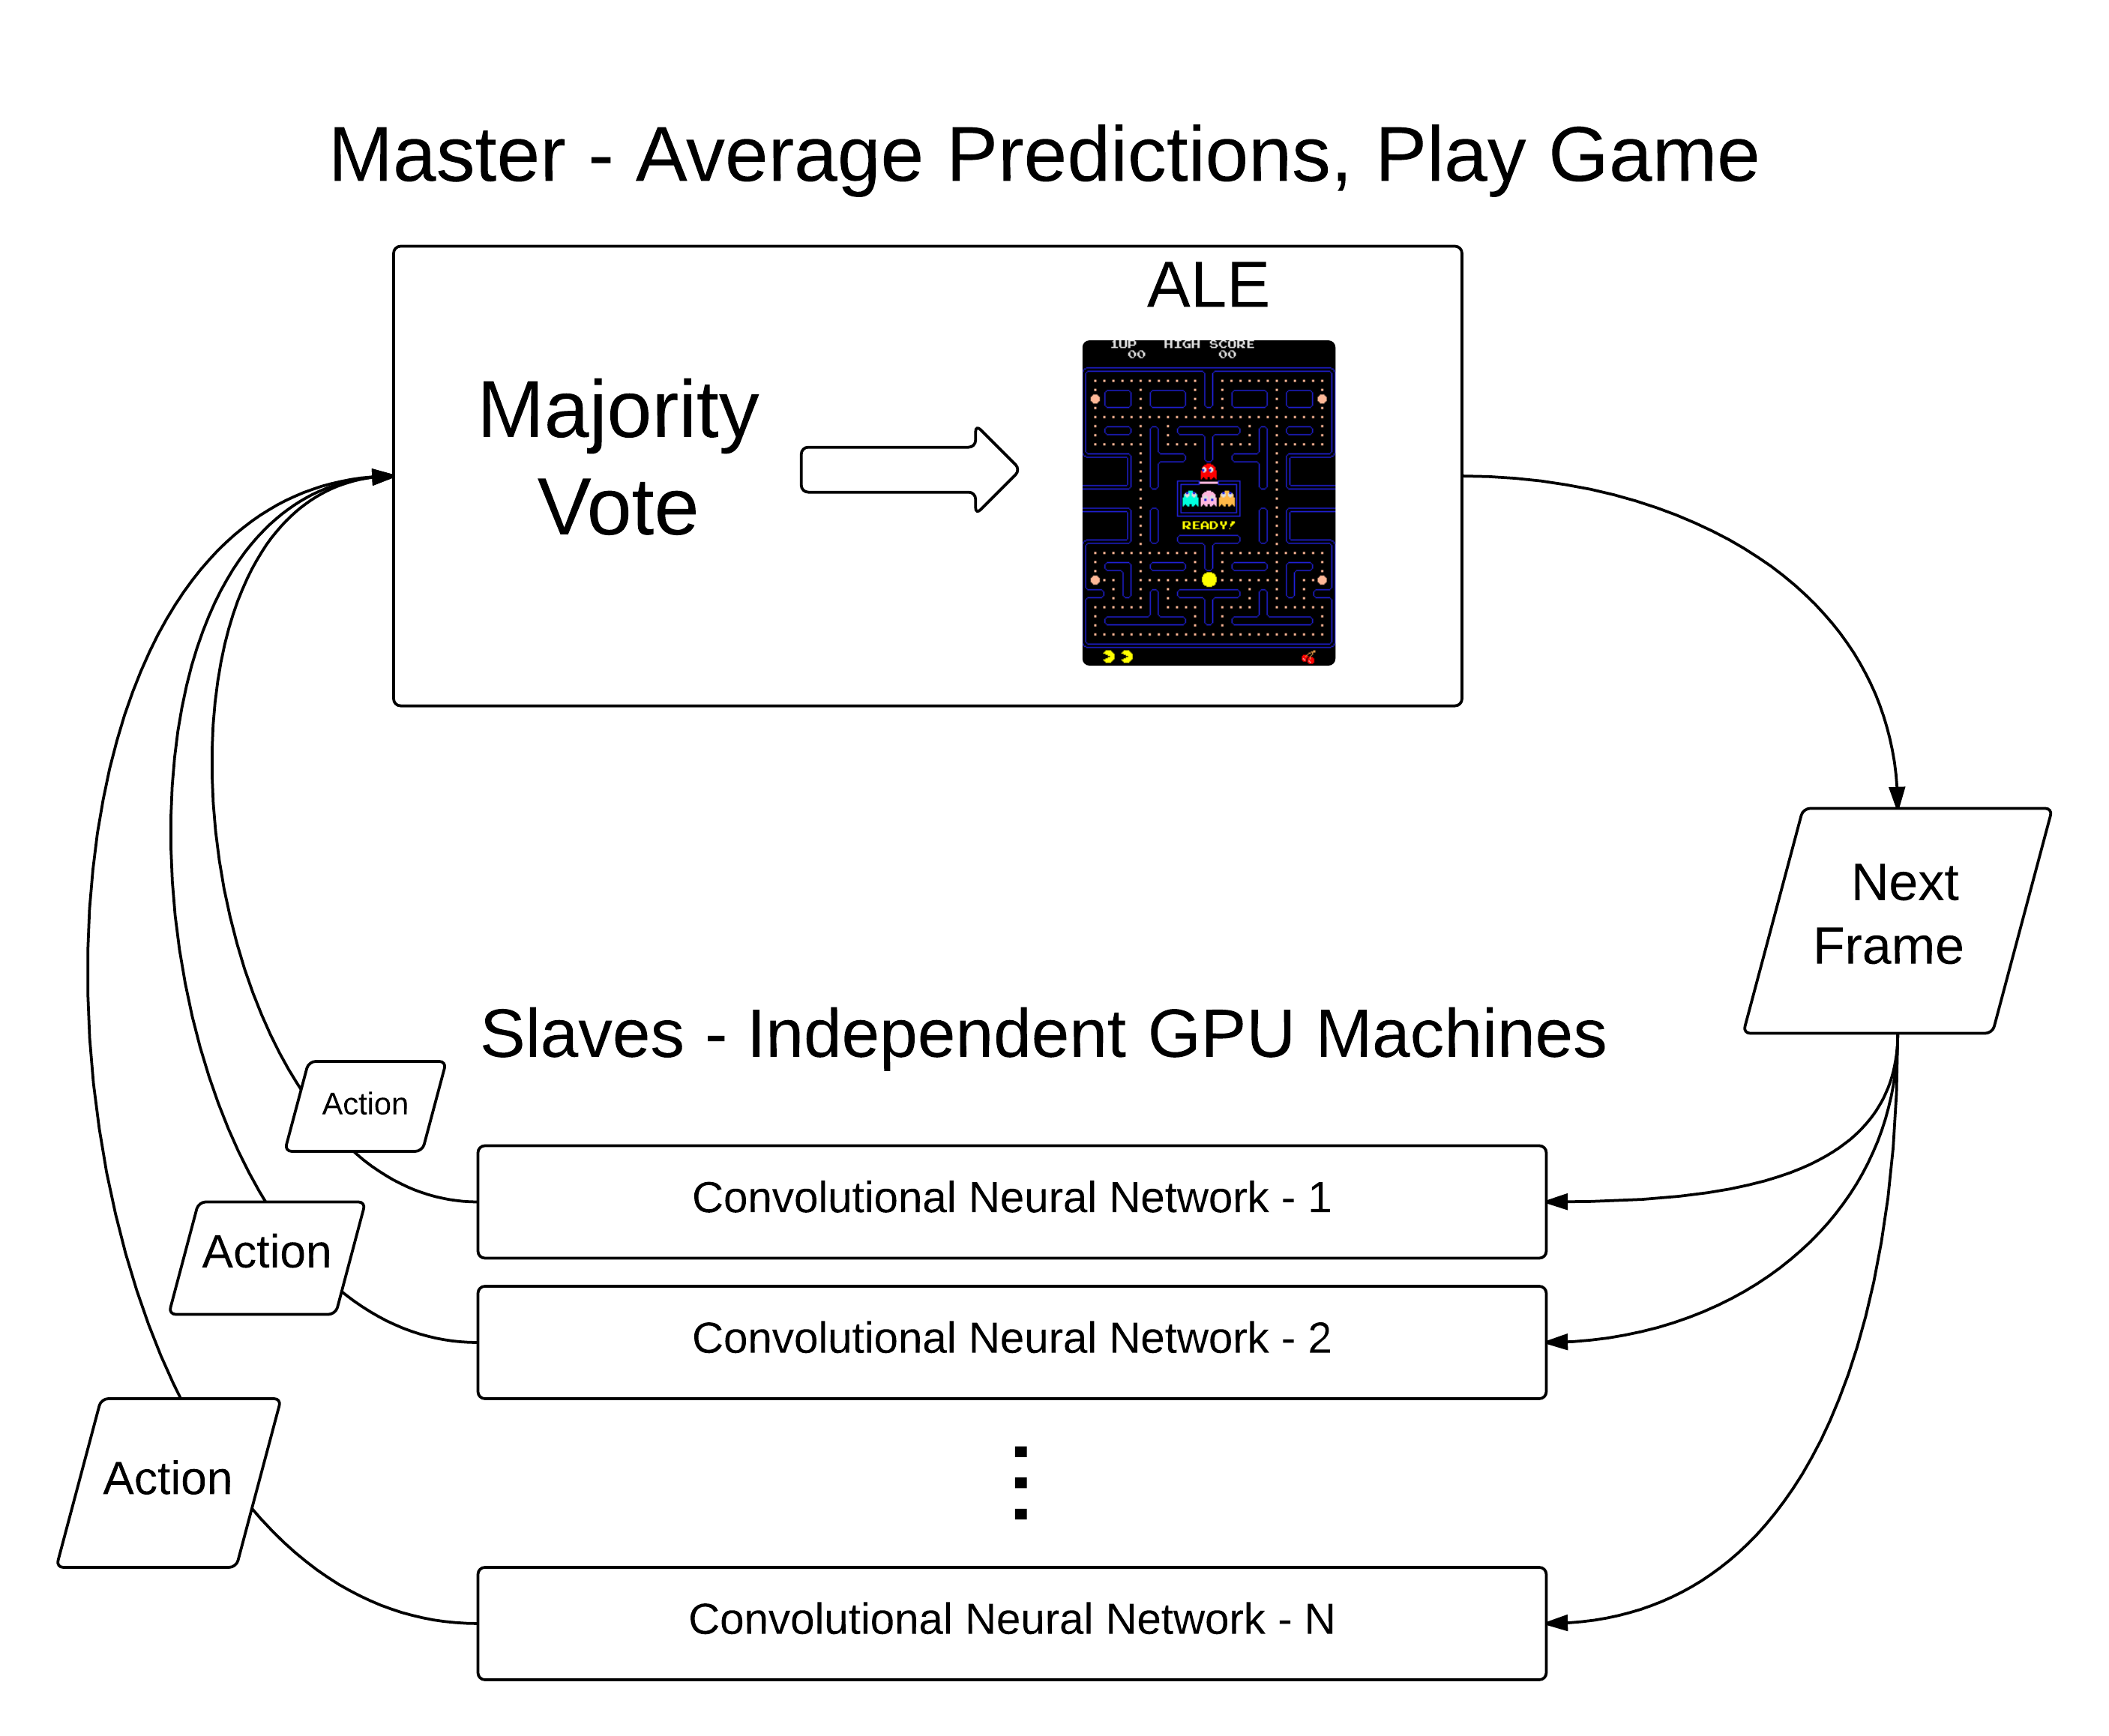
\includegraphics[width=1.0\textwidth]{arch}
%\fbox{\rule[-.5cm]{0cm}{4cm} \rule[-.5cm]{4cm}{0cm}}
\end{center}
\caption{Cluster Architecture}
\end{figure}


\begin{table}[H]
\caption{TODO: Title}
\label{sample-table}
\begin{center}
    \begin{tabular}{l | ccc}
        {\bf Config} & \multicolumn{1}{c}{\bf Space}  & \multicolumn{1}{c}{\bf Breakout} & \multicolumn{1}{c}{\bf Pacman} \\
        \\ \hline \\
        3x6     &6 &5 &5 \\
        3x10    &6 &5 &5 \\
        3x18    &6 &5 &5 \\
    \end{tabular}
\end{center}
\end{table}


\section{Results}

\begin{figure}[H]
\begin{center}
%\framebox[4.0in]{$\;$}
%\includegraphics[width=1.0\textwidth]{filename}
\fbox{\rule[-.5cm]{0cm}{4cm} \rule[-.5cm]{4cm}{0cm}}
\end{center}
\caption{Effect of Ensemble Size on Performance.}
\end{figure}

\begin{figure}[H]
\begin{center}
%\framebox[4.0in]{$\;$}
%\includegraphics[width=1.0\textwidth]{filename}
\fbox{\rule[-.5cm]{0cm}{4cm} \rule[-.5cm]{4cm}{0cm}}
\end{center}
\caption{Effect of Training Time on Ensembles.}
\end{figure}


\section{Conclusion}
\subsubsection*{Acknowledgments}
Thanks Mom

\subsubsection*{References}

\small{
[1] Watkins, Christopher JCH, and Peter Dayan. "Q-learning." {\it Machine learning} 8.3-4 (1992): 279-292.

[2] Mnih, Volodymyr, et al. "Human-level control through deep reinforcement 
learning." {\it Nature} 518.7540 (2015): 529-533.

[3] Krizhevsky, Alex, Ilya Sutskever, and Geoffrey E. Hinton. "Imagenet classification with deep convolutional neural networks." {\it Advances in neural information processing systems}. 2012.

[4] Szegedy, Christian, et al. "Going deeper with convolutions." {\it arXiv preprint arXiv:1409.4842} (2014).

[5] Simonyan, Karen, and Andrew Zisserman. "Very deep convolutional networks for large-scale image recognition." {\it arXiv preprint arXiv:1409.1556} (2014).

[6] He, Kaiming, et al. "Delving deep into rectifiers: Surpassing human-level performance on imagenet classification." {\it arXiv preprint arXiv:1502.01852} (2015).

[7] Sermanet, Pierre, et al. "Overfeat: Integrated recognition, localization and detection using convolutional networks." {\it arXiv preprint arXiv:1312.6229} (2013).

[8] Breiman, Leo. "Bagging predictors." {\it Machine learning} 24.2 (1996): 123-140.

[9] Schwenk, Holger, and Yoshua Bengio. "Boosting neural networks." {\it Neural Computation} 12.8 (2000): 1869-1887.

[10] Ha, Kyoungnam, Sungzoon Cho, and Douglas MacLachlan. "Response models based on bagging neural networks." {\it Journal of Interactive Marketing} 19.1 (2005): 17-30.

[11] Krizhevsky, Alex. "One weird trick for parallelizing convolutional neural networks." {\it arXiv preprint arXiv}:1404.5997 (2014).

[12] Ioffe, Sergey, and Christian Szegedy. "Batch normalization: Accelerating deep network training by reducing internal covariate shift." {it arXiv preprint arXiv}:1502.03167 (2015).

[] Dean, Jeffrey, et al. "Large scale distributed deep networks." {\it Advances in Neural Information Processing Systems}. 2012.

[] Collobert, Ronan, Koray Kavukcuoglu, and Clément Farabet. "Torch7: A matlab-like environment for machine learning." {\it BigLearn, NIPS Workshop}. No. EPFL-CONF-192376. 2011.
}

\end{document}
